\subsection{Student}
The student experience from start to finish is a much more fluid process than before, take for an example a student Jack who wishes to sign up to help find himself a job for his third year compulsary industrial placement.
  \subsubsection{Sign Up}
    The first thing Jack must do is sign up to CPP 2.0, under Imperial College's organisation. He can then choose the relevant departments he is a member of (in his case only Computing), enter a valid email address, password and password confirmation.

    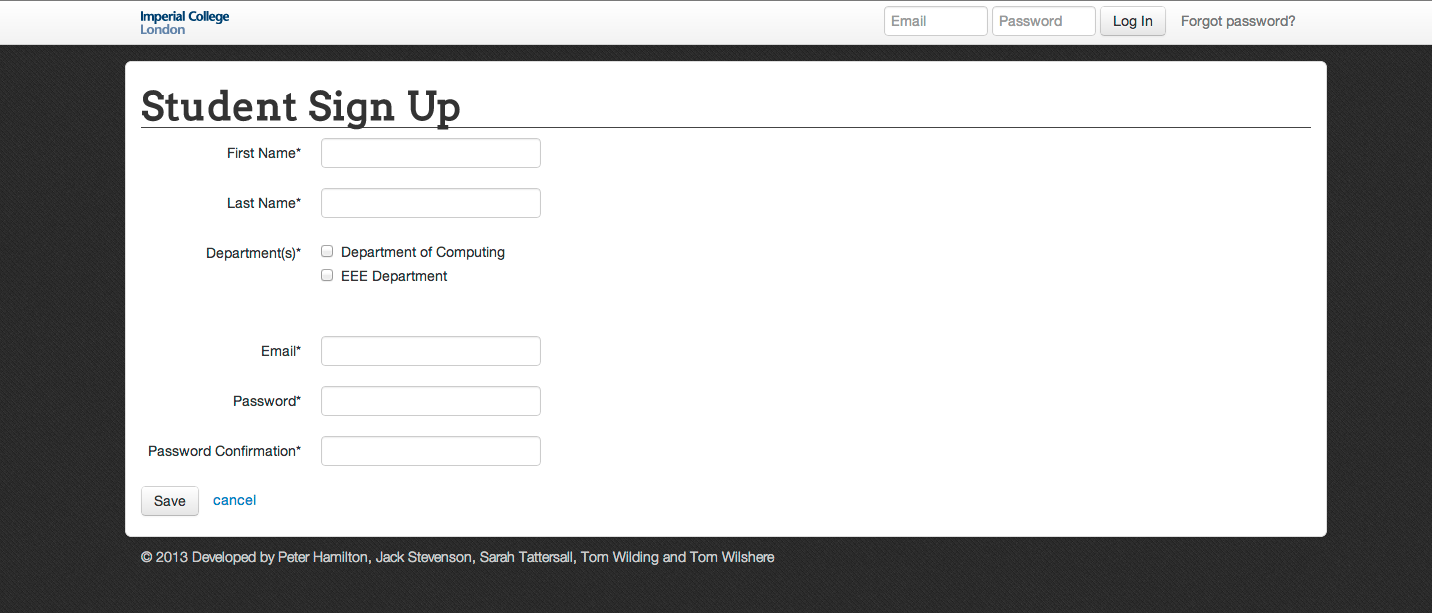
\includegraphics[scale=0.3]{images/user_experiences/student/sign_up_page}

    In order to sign up Jack must have a valid Imperial email address which will be identified if he uses his home address. We have used this as a technique to only allow students from a particular organisation to sign up.

    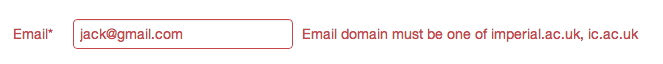
\includegraphics[scale=0.5]{images/user_experiences/student/invalid_email}

    Finally when all of Jack's details are correct he procedes to his dashboard. In order to not waste companies time with students that have not filled in their minimal details we deactivate a students profile on creation. A deactivated profile will not show up in company searches and required at minimum a year, degree, status and CV to be revealed to companies. 
    Jack is made aware of this via a drop down notifier on the page load which tells them so, to make it even more obvious we have decided to grey out student's profile and provide a mesage that their profile is de-activated at the top too.

    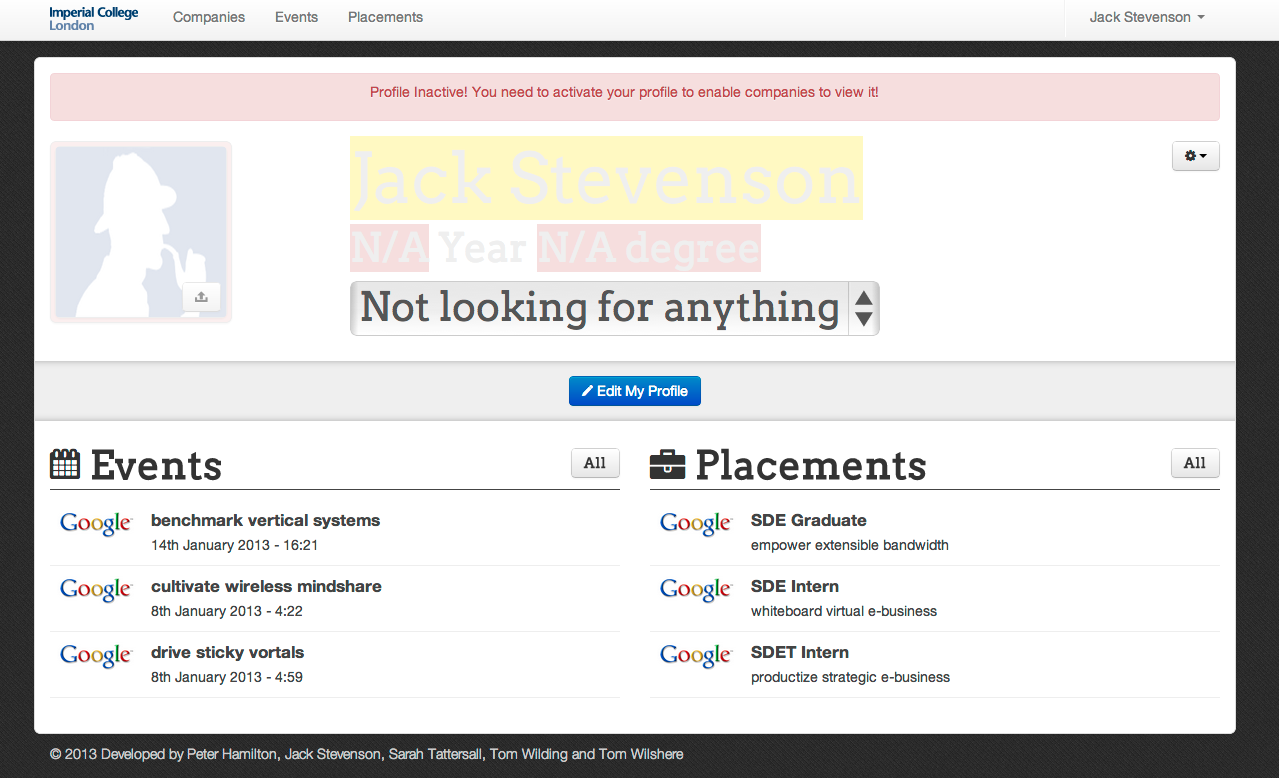
\includegraphics[scale=0.3]{images/user_experiences/student/sign_up_deactivate}

    Jack can then fill in his details and activate his profile ready to be found by a company.
    A complete example of which can be seen below.

    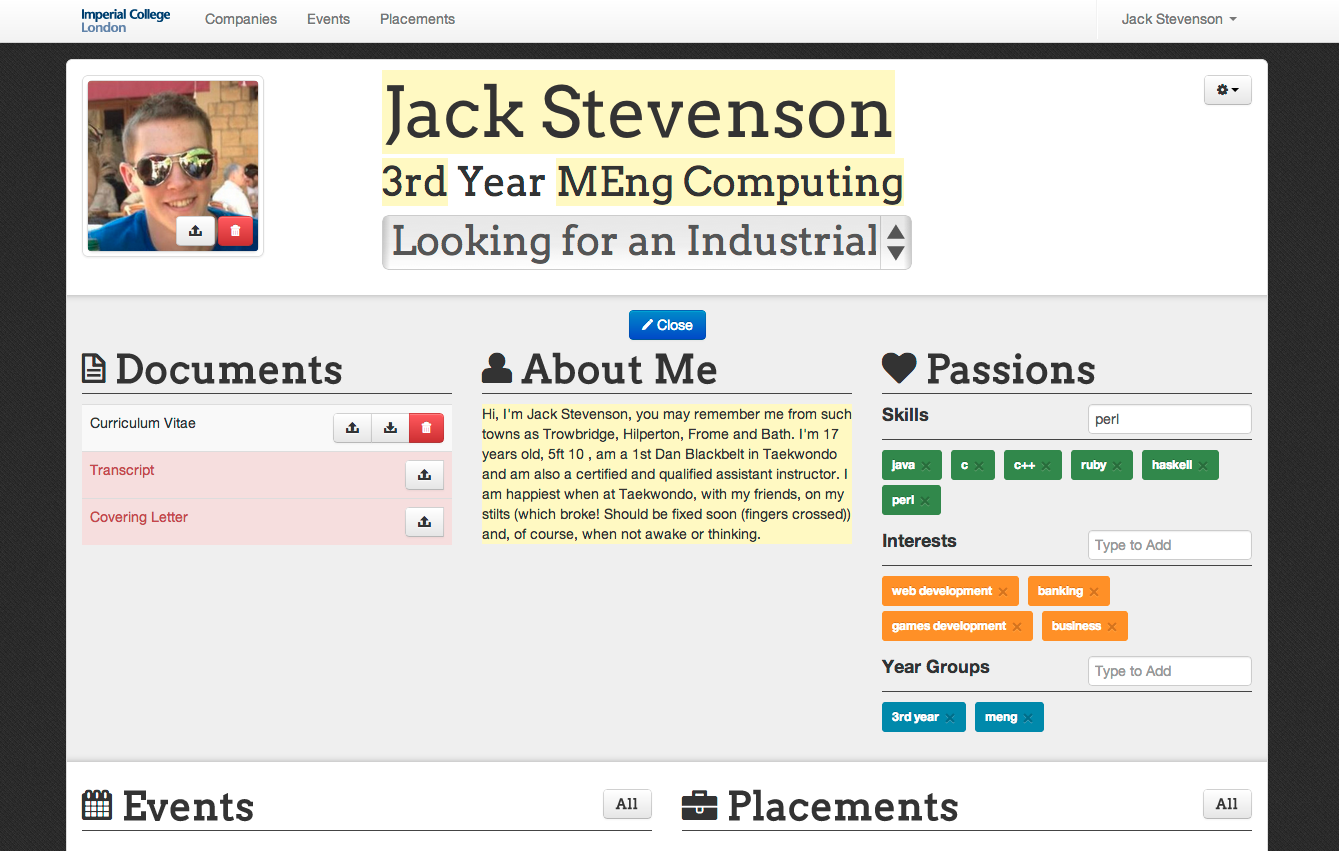
\includegraphics[scale=0.3]{images/user_experiences/student/edit_complete}

    In order to make modifying his profile easy and intuative, we have a number of helpful features on the page:
    \begin{itemize}
      \item Sections which have not been filled in or documents that are not uploaded are highligthed in red to notify the user that they are missing, and to encourage them to add them.
      \item To encourage all students to make use of the same degree type and passion tags we have added drop down suggestions for when a student starts typing in these areas.
      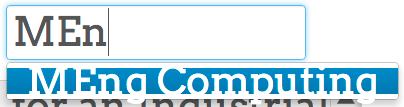
\includegraphics[scale=0.5]{images/user_experiences/student/edit_suggestions}
      \item So that the student realises they can use inline editing on their main information we have added tool tips that pop up whenever a user places their mouse over an item, and have also highligted these in yellow.
      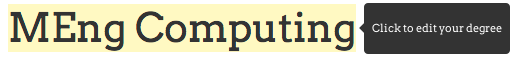
\includegraphics[scale=0.5]{images/user_experiences/student/edit_degree_tooltip}
    \end{itemize} 

    Jack also has an account settings page which can be accessed by the dropdown arrow on his name which features on the navigation bar. All that can be done is visible from the picture below. Here Jack can express if there are any skills he does not wish to receive emails about when looking for a placement.

    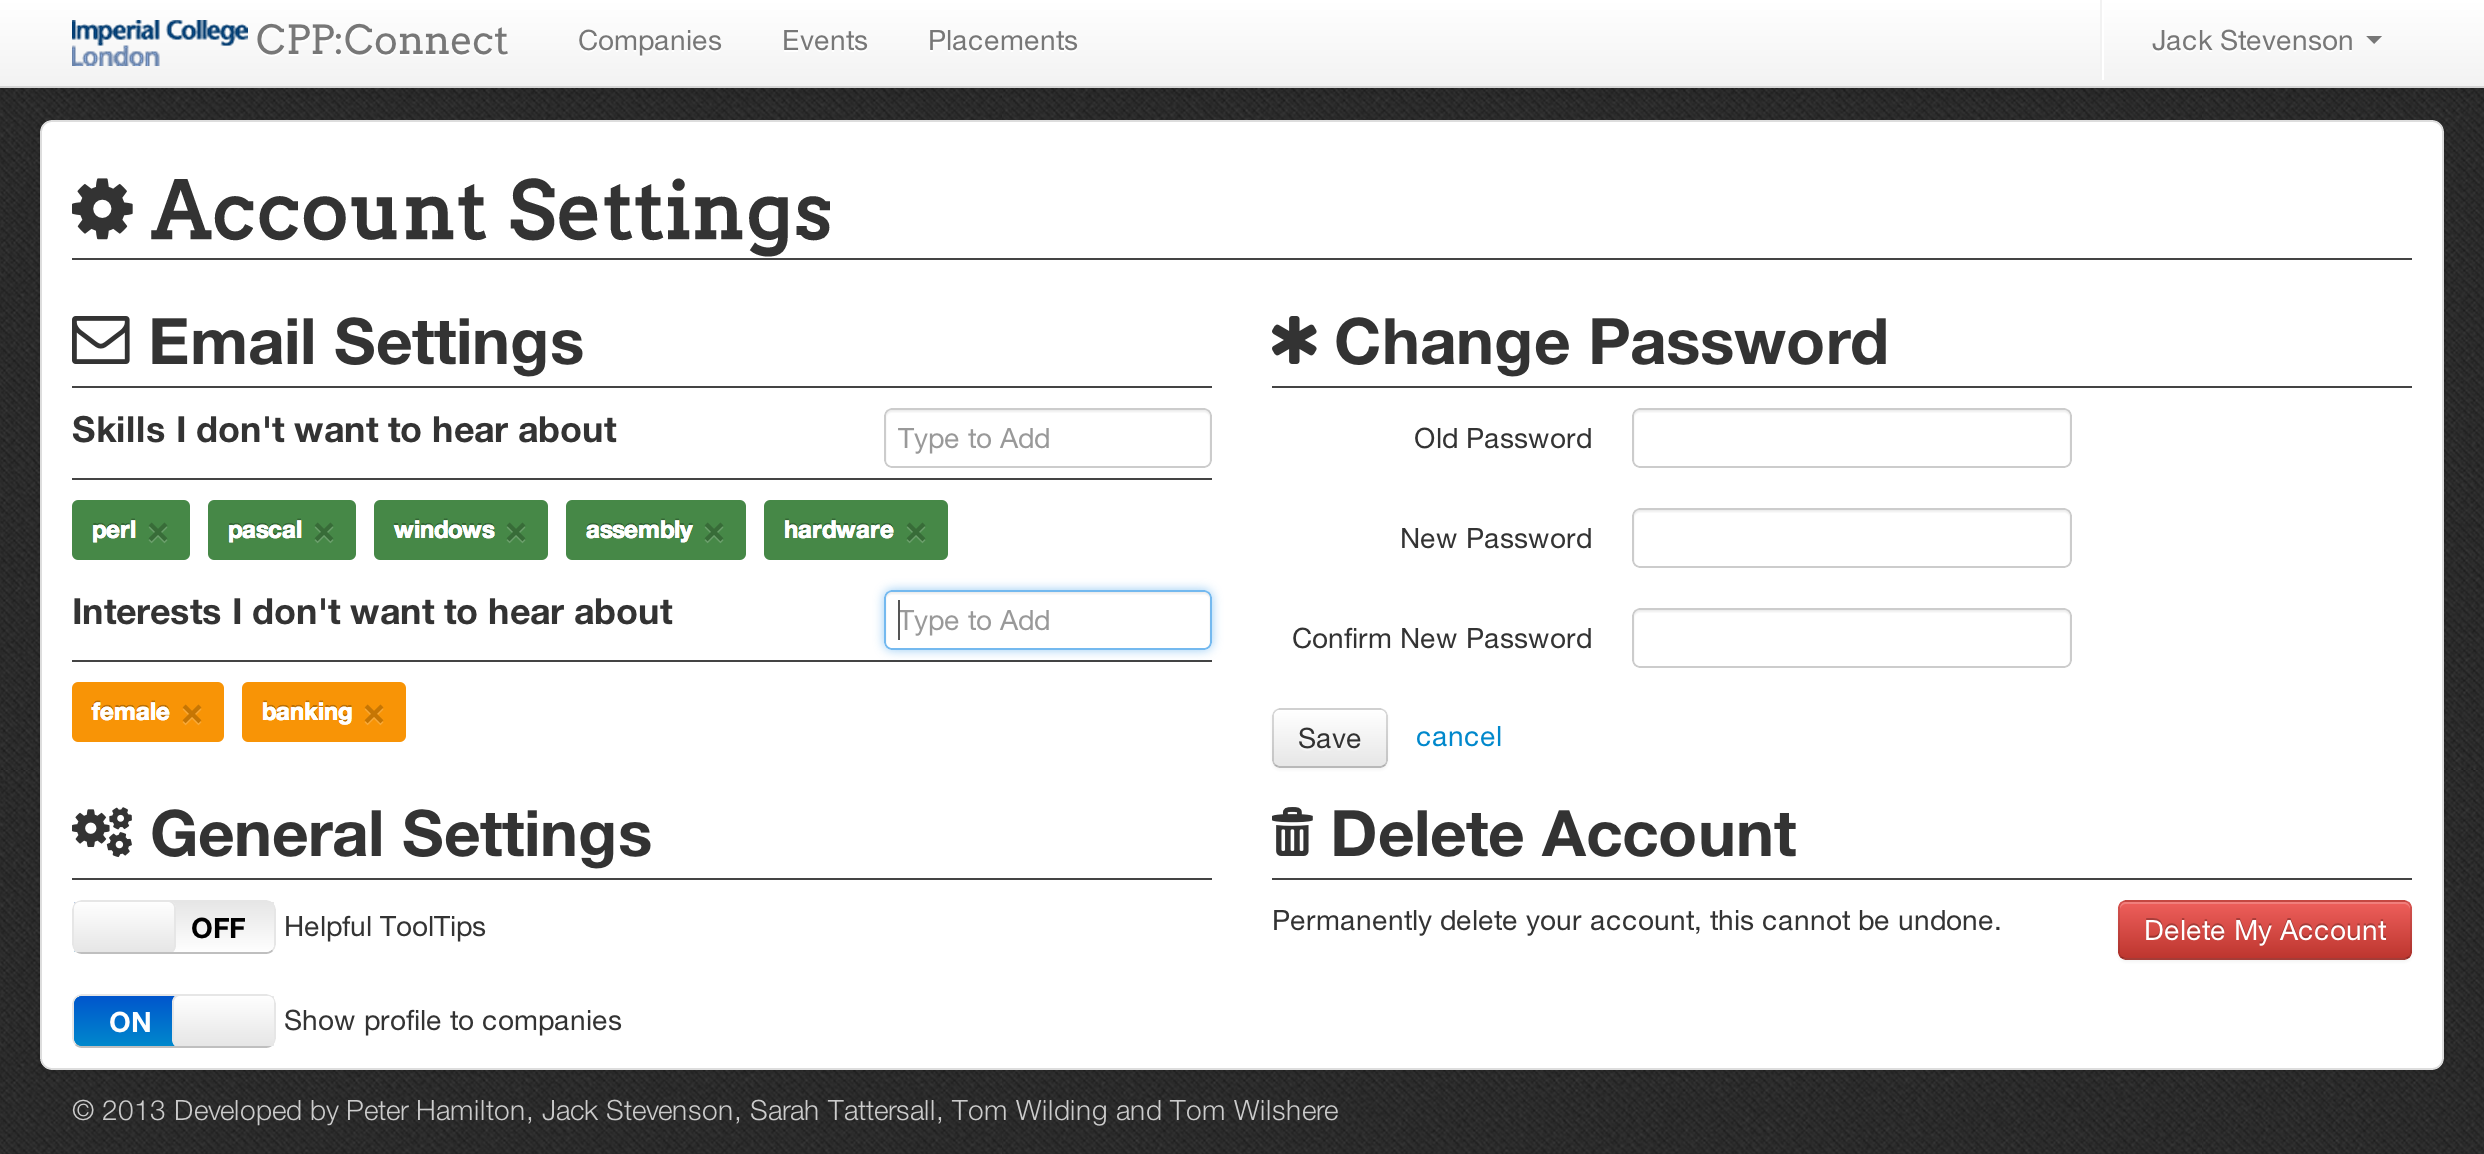
\includegraphics[scale=0.3]{images/user_experiences/student/account_settings}

    When logged in and looking at his profile, Jack can see new events and placements that have recently been advertised. By attending events students often make better contacts with companies than applying online and so Jack may wish to view these events by clicking on any of these or the all button. He can then sign up to attend events, and receive specific email notifications about them.
    He can also browse advertised placements and send an email to any companies that advertise one he is really keen about.

    If Jack is not interested, or does not wish to be contacted by specific companies he can choose to blacklist them. For example if Jack is not interested in a career with Amazon he can search for them on the companies list and then block (or faviourte instead) them with the icons in the corner. 

    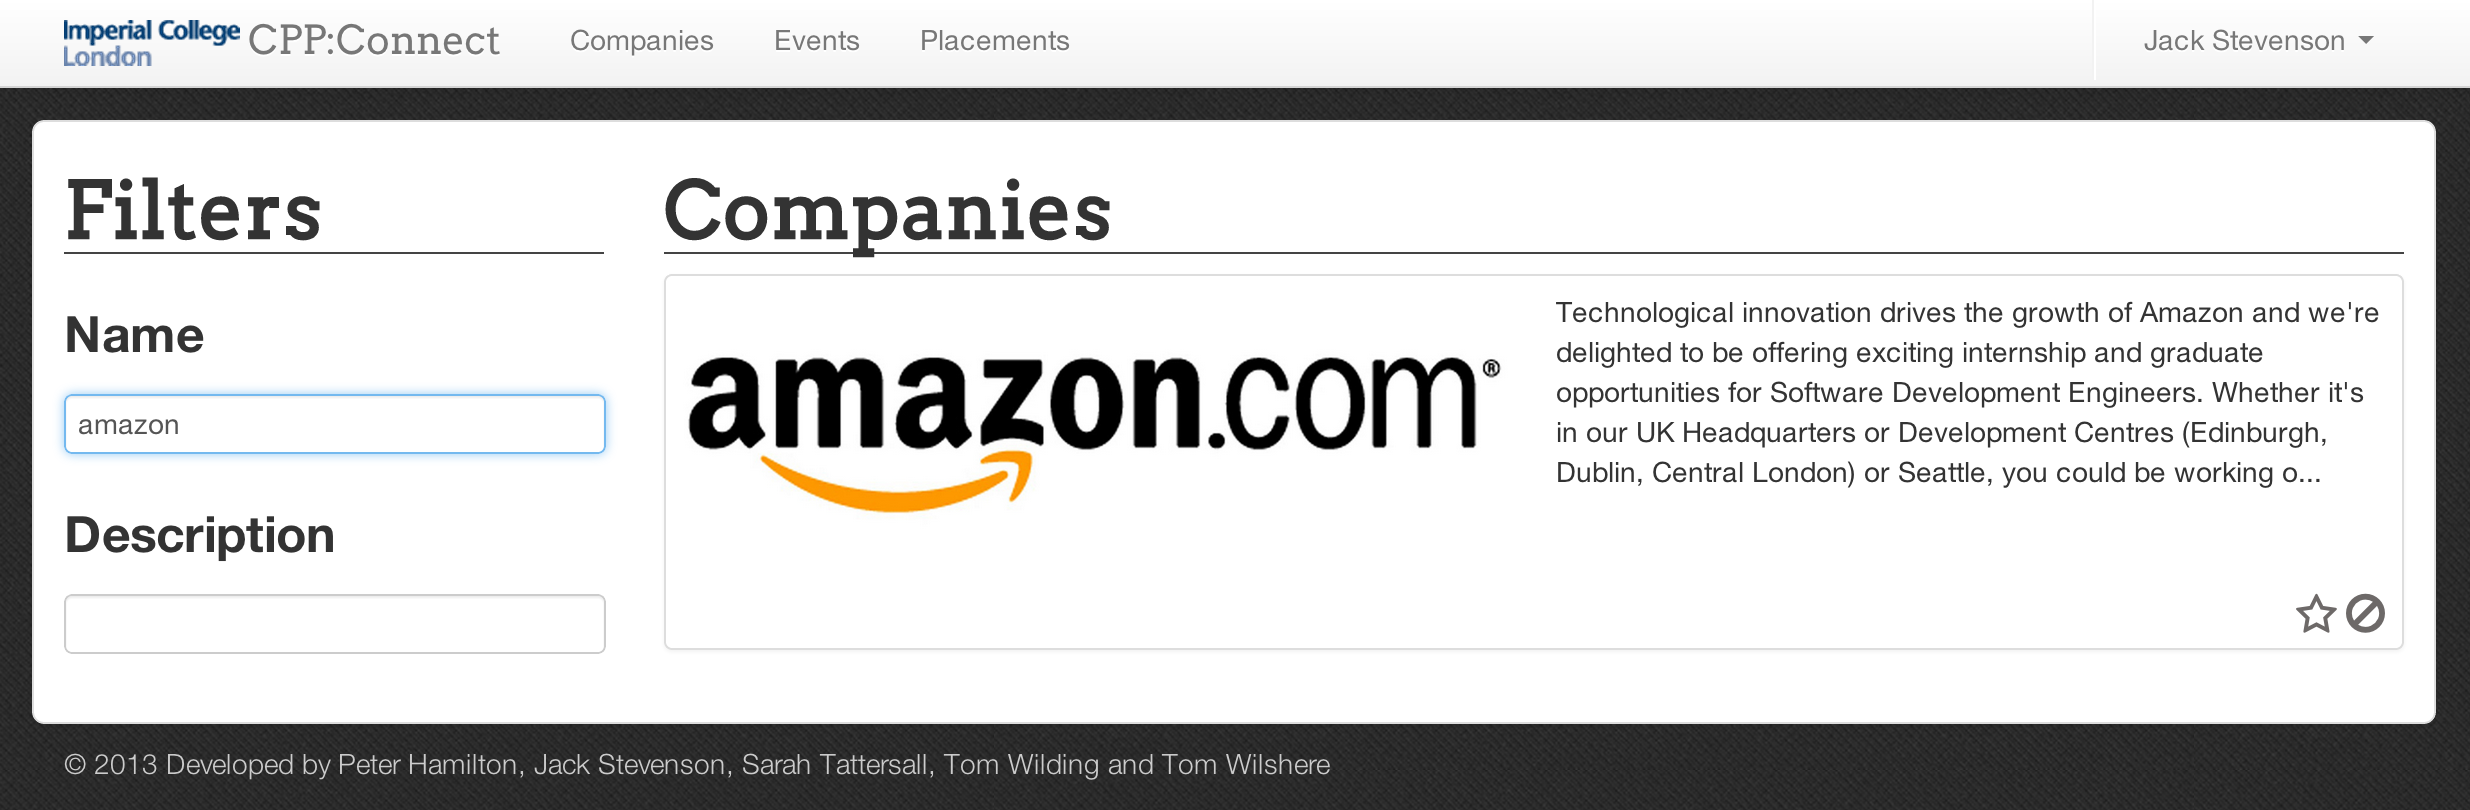
\includegraphics[scale=0.3]{images/user_experiences/student/block_amazon}

    %TODO Section about events page and all events, however not really ready yet.

